%\begin{frame}
%  \frametitle{What is a Molten Salt Reactor (MSR)?}
%	\begin{itemize}
%	  \item Advanced nuclear reactor fueled by fissile
%		material dissolved in a molten salt mixture
%	  \item In most MSR designs, the fuel salt mixture doubles as the primary coolant for the
%        reactor
%	  \item Both thermal- and fast-spectrum configurations are viable
%	\end{itemize}
%	\begin{figure}
%	  \centering
%	  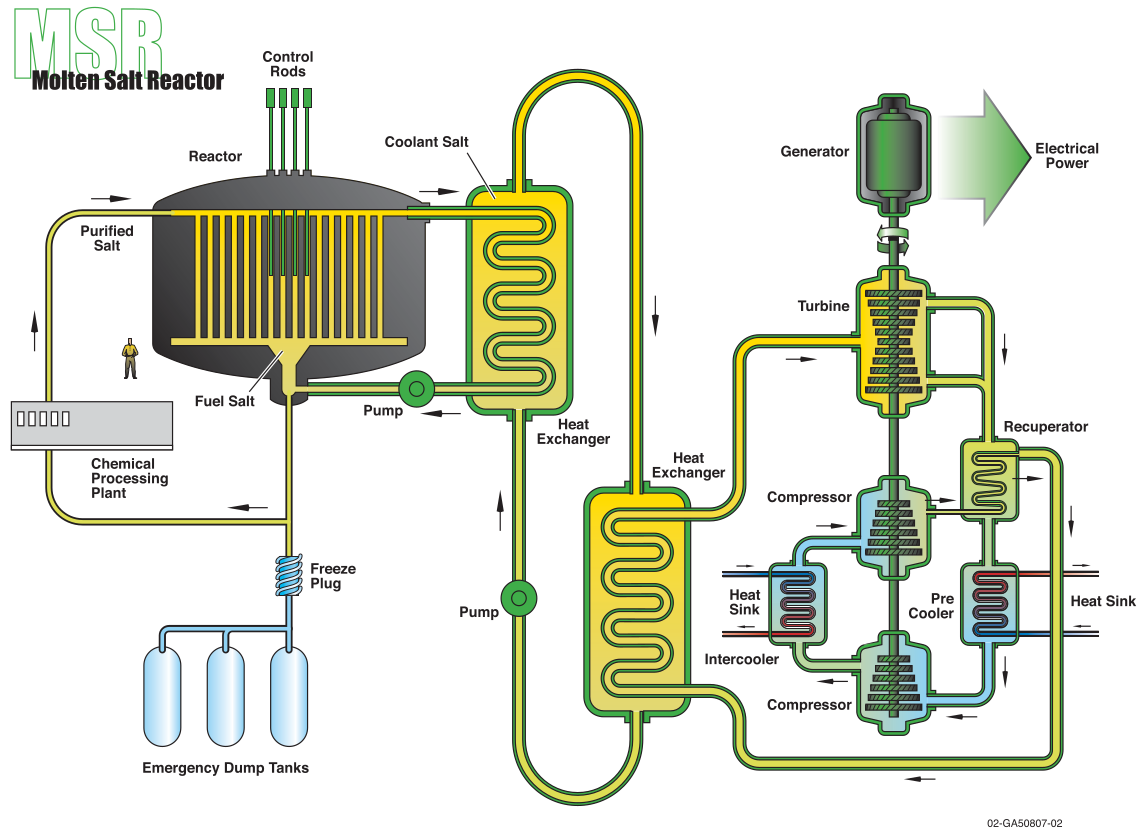
\includegraphics[width=.5\textwidth]{./images/msr}
%      \caption{Schematic diagram of a general channel-type MSR concept
%      \cite{u.s._doe_nuclear_energy_research_advisory_committee_technology_2002}.}
%	  \label{fig:msr}
%	\end{figure}
%\end{frame}

\begin{frame}
  \frametitle{Molten Salt Reactor Modeling \& Simulation}
  \textbf{What is a Molten Salt Reactor (MSR)?}
  \begin{itemize}
	\item MSRs are advanced nuclear reactors fueled by fissile
	  material dissolved in a molten salt mixture.
    \item While modeling MSRs is not necessarily more difficult than modeling solid-fueled
      reactors, we must adapt our software tools to accurately model phenomena unique to MSRs.
  \end{itemize}

  \textbf{Phenomena that pose challenges for MSR modeling}
  \begin{itemize}
	\item Strong multiphysics interactions involving neutron flux, temperature, and flow in the
      reactor core
	  \begin{itemize}
		\item Strong temperature feedback due to thermal expansion of liquid fuel salt
		\item Movement of \glspl{DNP} along primary coolant loop
        \item Advection-dominated heat transfer
	  \end{itemize}
    \item Loss of delayed neutrons to out-of-core decay
    \item Complex turbulent flow effects in MSRs
  \end{itemize}
\end{frame}

